\chapter{Agent Engineering --- From Prototype to Production}
\label{ch:agent-engineering}

\begin{quote}
\itshape
``Building an agent that works in a demo takes a weekend. Building an agent that works in production takes six months. The difference is entirely engineering.''
\end{quote}

\vspace{0.5cm}

\noindent
Chapter~\ref{ch:agents} covered the conceptual foundations of AI agents: architectures, reasoning paradigms, memory systems, and guardrails. This chapter is about the unglamorous engineering work that transforms a prototype agent into a production system: deterministic scaffolding around probabilistic reasoning, structured error handling for tools that can fail in novel ways, observability for systems whose internal reasoning is opaque, and testing strategies for agents whose behavior is non-deterministic by design.

The central thesis of this chapter is that \textbf{production agents are 20\% LLM and 80\% traditional software engineering}. The LLM provides the reasoning capability. Everything else---tool execution, state management, error recovery, observability, cost control, and safety---is conventional (if challenging) engineering. Figure~\ref{fig:agent-skeleton} shows the components of the production agent skeleton.

\begin{figure}[htbp]
\centering
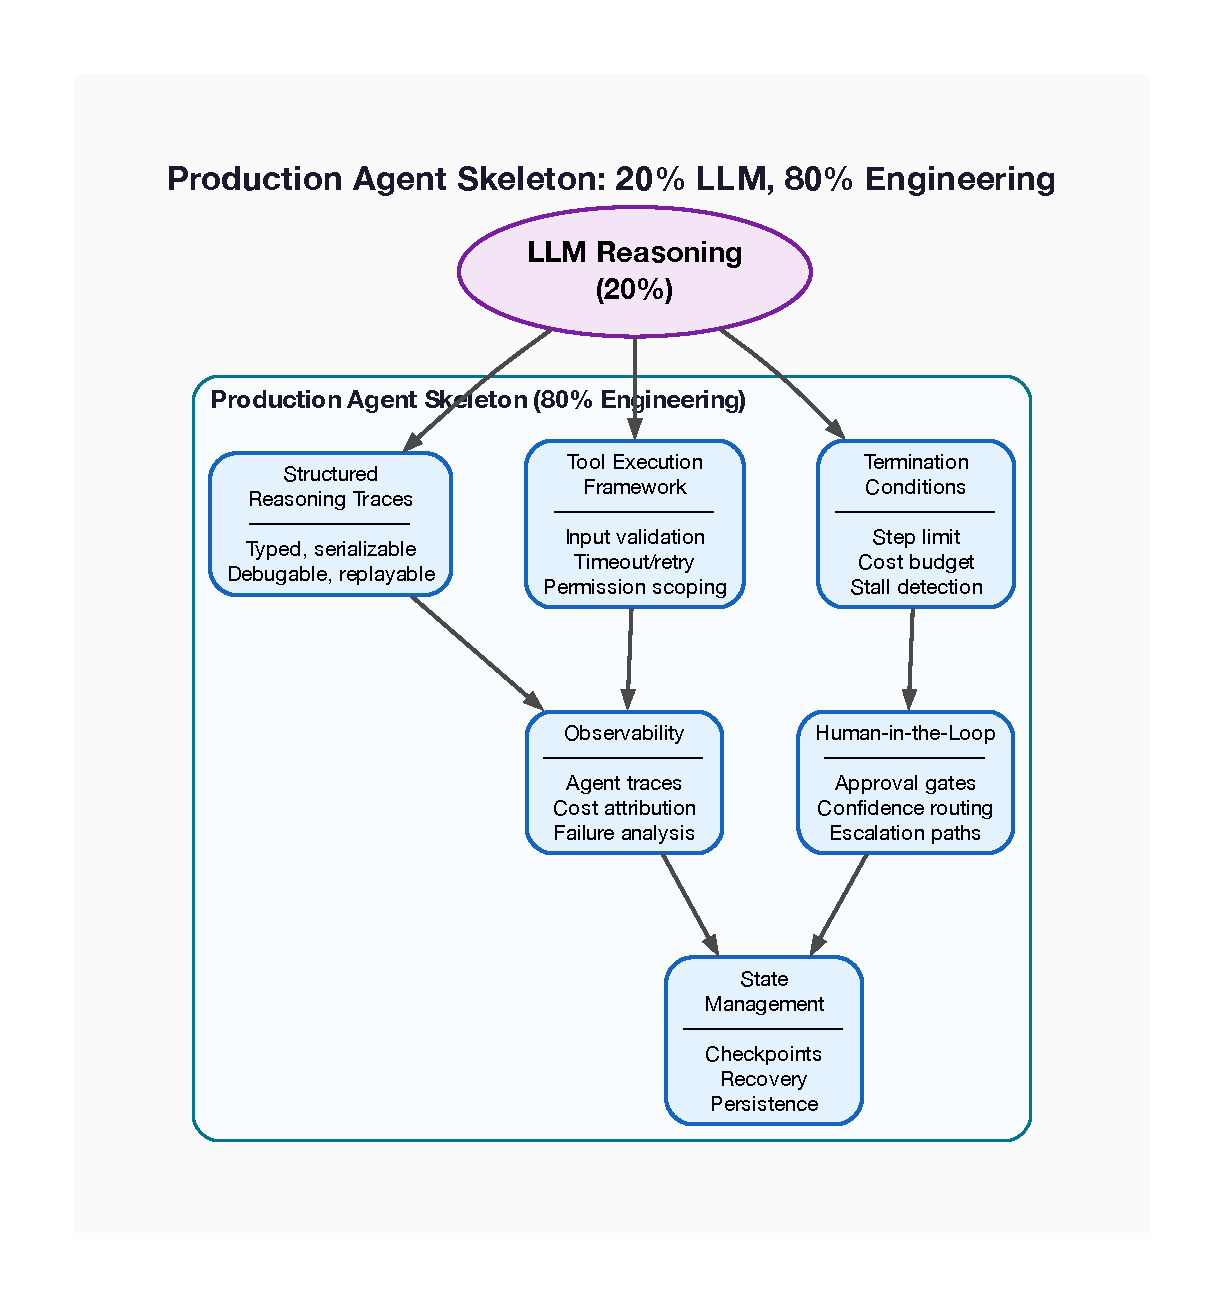
\includegraphics[width=\textwidth]{diagrams/compiled/ch13/agent-skeleton.pdf}
\caption{The production agent skeleton: 20\% LLM reasoning surrounded by 80\% engineering infrastructure}
\label{fig:agent-skeleton}
\end{figure}


\section{The Production Agent Skeleton}

Every production agent, regardless of its specific task, shares the same structural requirements. We call this the ``agent skeleton''---the infrastructure that must exist before you write a single line of agent logic.

\subsection{Structured Reasoning Traces}

The most important engineering decision in agent development: \textbf{every reasoning step must be a structured, serializable object}. Not a string. Not a log line. A typed data structure that can be inspected, stored, queried, and replayed.

This enables:

\begin{itemize}[leftmargin=*]
    \item \textbf{Debugging}: When an agent produces a wrong answer, you can inspect the exact reasoning chain---which tools it called, what results it received, and how it interpreted those results
    \item \textbf{Auditing}: For regulated industries, you need a complete, immutable record of every decision the agent made and why
    \item \textbf{Replay}: Given a stored reasoning trace, you can re-execute the agent from any checkpoint with different parameters (time-travel debugging)
    \item \textbf{Evaluation}: Automated evaluation of intermediate reasoning steps, not just final outputs
\end{itemize}

This is the Event-Sourced Agent pattern from Chapter~\ref{ch:app-architecture}: every \textsc{Observe} $\to$ \textsc{Think} $\to$ \textsc{Act} cycle is persisted as an immutable event.


\subsection{Tool Execution Framework}

Tools are the bridge between the LLM's reasoning and the real world. In production, every tool execution must be wrapped in a framework that handles:

\begin{itemize}[leftmargin=*]
    \item \textbf{Input validation}: Validate tool arguments before execution. The LLM may hallucinate field names, use wrong types, or pass empty values.
    \item \textbf{Timeout and retry}: Every tool call has a timeout. Network requests get retries with exponential backoff. Database queries get statement timeouts.
    \item \textbf{Permission scoping}: Each agent should have the minimum permissions necessary. A customer support agent should not have database write access. A code generation agent should not have network access.
    \item \textbf{Output normalization}: Tool outputs must be normalized into a consistent format before being passed back to the LLM. Raw API responses, exception stack traces, and binary data must be summarized or truncated.
    \item \textbf{Cost tracking}: Every tool call has a cost (API fees, compute time, storage). Track cumulative cost per agent session.
\end{itemize}

\subsection{Termination Conditions}

An agent without explicit termination conditions will run forever (or until it hits a rate limit). Production agents must have:

\begin{enumerate}[leftmargin=*]
    \item \textbf{Goal completion}: The agent has achieved its stated objective (verified by a structured check, not by the agent's self-assessment)
    \item \textbf{Step limit}: Maximum number of reasoning cycles (typically 15--50 depending on task complexity)
    \item \textbf{Cost budget}: Maximum token or dollar spend per session
    \item \textbf{Time budget}: Wall-clock time limit
    \item \textbf{Error threshold}: Maximum consecutive errors before escalation
    \item \textbf{Semantic stall detection}: The Semantic Circuit Breaker pattern---if the agent's actions become repetitive (high cosine similarity between consecutive steps), autonomy is suspended
\end{enumerate}

\begin{cautionbox}[The Self-Assessment Trap]
Never rely on the agent's own judgment about whether it has completed its task. Agents are biased toward claiming success. Use external validation: run the test suite, check the database state, verify the API response. ``The agent said it's done'' is not a termination condition.
\end{cautionbox}


\section{Multi-Agent Systems in Production}

\subsection{When to Use Multiple Agents}

Single-agent systems are simpler, cheaper, and easier to debug. Use multiple agents only when:

\begin{itemize}[leftmargin=*]
    \item \textbf{Different expertise required}: A coding agent and a documentation agent need different system prompts, tools, and evaluation criteria
    \item \textbf{Separation of concerns}: A planning agent and an execution agent have different risk profiles and require different guardrails
    \item \textbf{Parallel work}: Multiple independent subtasks can be executed concurrently
    \item \textbf{Adversarial validation}: A generator agent and a critic agent (the Generator-Critic pattern) provide quality guarantees that a single agent cannot
\end{itemize}

\subsection{Inter-Agent Communication}

Use the Agent-to-Agent (A2A) protocol or a similar structured communication framework:

\begin{itemize}[leftmargin=*]
    \item \textbf{Agent Cards}: Each agent publishes a capability card describing what it can do, what inputs it accepts, and what outputs it produces
    \item \textbf{Task delegation}: Hierarchical routing---a coordinator agent decomposes a goal and assigns subtasks to specialist agents
    \item \textbf{Structured handoffs}: When one agent passes work to another, the handoff includes: the original goal, work completed so far, remaining tasks, and any constraints or context the receiving agent needs
    \item \textbf{Result aggregation}: The coordinator collects results from specialist agents, reconciles any conflicts, and synthesizes the final output
\end{itemize}

\subsection{Failure Modes in Multi-Agent Systems}

Multi-agent systems have unique failure modes:

\begin{itemize}[leftmargin=*]
    \item \textbf{Circular delegation}: Agent A delegates to Agent B, which delegates back to Agent A. Prevent with delegation depth limits.
    \item \textbf{Conflicting actions}: Two agents attempt to modify the same resource simultaneously. Prevent with explicit resource locking.
    \item \textbf{Context fragmentation}: Each agent has a partial view of the overall state. Prevent with a shared context store that all agents read from.
    \item \textbf{Cascading failures}: One agent's failure causes downstream agents to fail or hallucinate. Prevent with explicit error propagation and fallback strategies.
\end{itemize}


\section{Agent Observability}

Agent systems are the hardest software to debug because their behavior is non-deterministic, their reasoning is opaque, and their failures are often semantic rather than structural.

\subsection{The Agent Trace}

Every agent session should produce a structured trace that includes:

\begin{enumerate}[leftmargin=*]
    \item \textbf{Session metadata}: Start time, end time, total cost, total steps, termination reason
    \item \textbf{Reasoning chain}: Each Think step with the model's output, the parsed intent, and the selected action
    \item \textbf{Tool calls}: Each tool invocation with input arguments, output, latency, and cost
    \item \textbf{Context snapshots}: The contents of the context window at each step (what the model ``saw'' when making each decision)
    \item \textbf{Quality assessments}: Intermediate evaluation scores from judge models or structural validators
\end{enumerate}

\subsection{Trace Analysis}

Agent traces enable post-hoc analysis:

\begin{itemize}[leftmargin=*]
    \item \textbf{Failure analysis}: ``Why did the agent call the wrong API?'' Answer: because the retrieval step returned irrelevant documentation. Root cause: the query was ambiguous and the RAG system retrieved the wrong documents.
    \item \textbf{Efficiency analysis}: ``Why did this task take 47 steps?'' Answer: because the agent tried three different approaches before finding one that worked. Optimization: better planning or few-shot examples.
    \item \textbf{Cost attribution}: ``Why did this session cost \$2.40?'' Answer: because the agent included the full document (12K tokens) in every reasoning step. Optimization: summarize the document once and use the summary.
\end{itemize}


\section{Testing Agents}

Agent testing is fundamentally different from traditional software testing because agent behavior is non-deterministic and path-dependent.

\subsection{Unit Testing Agent Components}

Test the deterministic components in isolation:

\begin{itemize}[leftmargin=*]
    \item \textbf{Tool functions}: Each tool should have comprehensive unit tests, independent of the agent
    \item \textbf{Input validators}: Test that malformed tool arguments are caught before execution
    \item \textbf{Output parsers}: Test that model outputs are correctly parsed into structured actions
    \item \textbf{Termination conditions}: Test that step limits, cost budgets, and stall detection trigger correctly
\end{itemize}

\subsection{Scenario Testing}

End-to-end tests with curated scenarios:

\begin{itemize}[leftmargin=*]
    \item Define 50--100 representative tasks with expected outcomes
    \item Run each scenario multiple times (N=5) to account for non-determinism
    \item Score on: task completion (binary), quality (rubric), efficiency (steps taken), cost (tokens used)
    \item A scenario ``passes'' if the agent completes the task in $\geq$4 out of 5 runs with quality above threshold
\end{itemize}

\subsection{Adversarial Testing}

Test agent resilience against:

\begin{itemize}[leftmargin=*]
    \item \textbf{Prompt injection through tools}: Malicious content in tool outputs that attempts to hijack the agent's reasoning
    \item \textbf{Tool failures}: What happens when a tool returns an error, times out, or returns unexpected data?
    \item \textbf{Ambiguous goals}: What happens when the user's request is vague or contradictory?
    \item \textbf{Resource exhaustion}: Does the agent respect cost and step limits under all conditions?
\end{itemize}


\section{Human-in-the-Loop Patterns}

Production agents rarely operate fully autonomously. Human oversight is essential for high-stakes actions, uncertain situations, and quality assurance.

\subsection{Approval Gates}

Define which actions require human approval before execution:

\begin{itemize}[leftmargin=*]
    \item \textbf{Always approve}: Delete operations, financial transactions, customer communications, production deployments
    \item \textbf{Approve above threshold}: Actions estimated to cost more than a defined amount, actions affecting more than N records
    \item \textbf{Auto-approve}: Read operations, internal calculations, test executions, documentation updates
\end{itemize}

\subsection{Confidence-Based Routing}

Use the Confidence Gate pattern (Chapter~\ref{ch:app-architecture}):

\begin{itemize}[leftmargin=*]
    \item \textbf{High confidence ($>$0.9)}: Auto-execute and report results
    \item \textbf{Medium confidence (0.6--0.9)}: Execute but flag for human review within 24 hours
    \item \textbf{Low confidence ($<$0.6)}: Queue for human decision before any action
\end{itemize}


\section{Chapter Summary}

\begin{enumerate}[leftmargin=*]
    \item \textbf{Production agents are 80\% engineering}: Tool execution, state management, error recovery, observability, and safety are all conventional engineering problems
    \item \textbf{Structure everything}: Reasoning traces, tool calls, and state transitions must be typed, serializable, and stored
    \item \textbf{Multi-agent systems need explicit coordination}: Agent Cards, structured handoffs, and delegation depth limits
    \item \textbf{Observability is essential}: Agent traces with reasoning chains, tool calls, and context snapshots enable debugging and optimization
    \item \textbf{Test at multiple levels}: Unit tests for components, scenario tests for end-to-end behavior, adversarial tests for resilience
    \item \textbf{Human-in-the-loop by default}: Approval gates and confidence-based routing, not full autonomy
\end{enumerate}

\begin{keytakeaway}
The gap between a demo agent and a production agent is entirely engineering. Structure your reasoning traces, wrap every tool call in a framework, enforce termination conditions, and never trust the agent's self-assessment. Production agents are conventional engineering problems with an unconventional component at their core.
\end{keytakeaway}
